\documentclass[a4paper,12pt,french]{article}

\usepackage[utf8]{inputenc}
\usepackage{roboto}
\usepackage{babel}
\usepackage{graphicx}
\usepackage{wrapfig}
\usepackage{index}
\makeindex

\begin{document}

\title{\Large{\textbf{LINFO1212 Final Project}}}
\author{Oscar Fally}
\date{November 5, 2019}

\maketitle
\tableofcontents
\setcounter{page}{0}

\clearpage

\section{Besoins du client}

Pour ce projet, j'ai été en contact avec un ingénieur du son. Celui-ci étant désireux 
de créer un systême lui permettant de stocker les fichiers audio de ses clients sur le net. 
\par
Il a spécifié vouloir un site simple mais efficace, permettant de trier 
et d'éditer les informations des fichiers.
Afin d'avoir une certaine autonomie, chaque user doit pouvoir ajouter 
ses fichiers audio depuis l'interface utilisateur.

\section{Interface utilisateur}

\begin{figure}[ht]
\centering
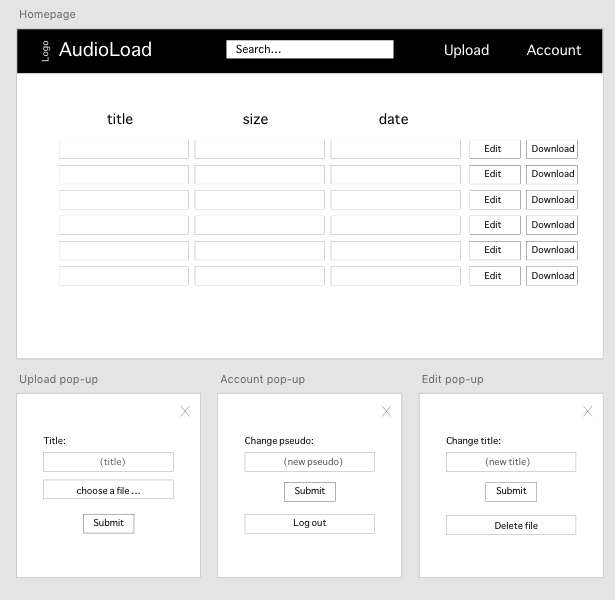
\includegraphics[width=13cm]{../prototype/homepage}
\caption{Homepage}
\end{figure}

Cette page est la page principale du site, affichant les fichiers audio de la base de données.
Trois actions sont possibles dans la barre de navigation:

\begin{itemize}
	\item ajouter un nouveau fichier
	\item changer de pseudo/se deconnecter
	\item changer le titre d'un fichier/le supprimer
\end{itemize}

Ces actions sont réalisées au sein de fenêtres pop-up apparaissant par dessus la homepage.

\begin{figure}[ht]
\centering
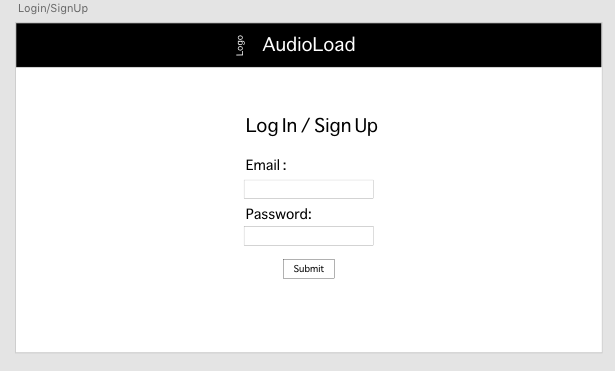
\includegraphics[width=13cm]{../prototype/login}
\caption{Log In / Sign Up}
\end{figure}

La seconde page est la première page qui apparait si aucune session user n'est trouvée.
Simple et directe, elle permet de se connecter où de créer un nouvel utilisateur si l'adresse mail n'existe pas encore dans la database.

\section{Architecture du système}

Le projet sera déployé sur un backend NodeJS/Express, 
permettant au front-end (Vue.JS ou Bootstrap, à définir) 
de communiquer avec une base de donnée MongoDB.
\par
Cette stack permettant une efficacité correcte en cas de besoin de scalability.
\section{Base de donnée}

La base de données MongoDB contiendra deux type de données essentiels permettant le bon fonctionnement du site:
\begin{itemize}
	\item \string[login - mot de passe - email - date] des users
	\item \string[user - titre - size - date - data] des fichiers audio
\end{itemize}

\section{Fonctionnalité de recherche}

Un user connecté peut rechercher des fichiers audio lui appartenant 
dans la base de données via la barre de recherche au centre du header, 
pour ensuite les télécharger ou les modifier.

\end{document}
